%%%%%%%%%%%%%%%%%%%%%%%%%%%%%%%%%%%%
% Header                           %
%%%%%%%%%%%%%%%%%%%%%%%%%%%%%%%%%%%%
% 
% Revisions: 2017-04-10 Martin R�del <martin.raedel@dlr.de>
%                       Initial draft
%               
% Contact:   Martin R�del,  martin.raedel@dlr.de
%            DLR Composite Structures and Adaptive Systems
%          
%                                 __/|__
%                                /_/_/_/  
%            www.dlr.de/fa/en      |/ DLR
% 
%%%%%%%%%%%%%%%%%%%%%%%%%%%%%%%%%%%%
% Content                          %
%%%%%%%%%%%%%%%%%%%%%%%%%%%%%%%%%%%%

\levelstay{\idxPDKwBondFilters}
\label{sec:Peridigm:QRG:Discretization:Tools:BondFilters}
\myindex[\idxPDKeywordName]{\idxPDKwBondFilters}

\leveldown{Description}

A method to omit bonds in the discretization.

\levelstay{Code}

Dependent on the type of discretization the following classes are used:

\begin{itemize}[noitemsep]
  \item from \texttt{src/io/discretization/}:
  \begin{itemize}[noitemsep]
    \item \texttt{Peridigm\_AlbanyDiscretization.cpp}
    \item \texttt{Peridigm\_AlbanyDiscretization.hpp}
    \item \texttt{Peridigm\_ExodusDiscretization.cpp}
    \item \texttt{Peridigm\_ExodusDiscretization.hpp}
    \item \texttt{Peridigm\_PdQuickGridDiscretization.hpp}
    \item \texttt{Peridigm\_PdQuickGridDiscretization.cpp}
    \item \texttt{Peridigm\_TextFileDiscretization.hpp}
    \item \texttt{Peridigm\_TextFileDiscretization.cpp}
  \end{itemize}
\end{itemize}

All extend the super-class

\begin{itemize}[noitemsep]
  \item \verb+/src/io/discretization/Peridigm_Discretization.cpp+
  \item \verb+/src/io/discretization/Peridigm_Discretization.hpp+
\end{itemize}

Each class uses the method from the super-class :

\verb+PeridigmNS::Discretization::createBondFilters+

\levelstay{Input parameters}

\leveldown{List}

\begin{tabularx}{\linewidth}{lcccX}
\toprule
Name                    & Type   & Required   & Default & Description           \\
\midrule
Type                    & string & \checkmark & - & ``\idxPDKwRectangularPlane'' \\
Normal\_X               & double & \checkmark & - & $\glssymbol{symb:scalar:coord:global:x}$-component of the cutting plane normal vector\\
Normal\_Y               & double & \checkmark & - & $\glssymbol{symb:scalar:coord:global:y}$-component of the cutting plane normal vector\\
Normal\_Z               & double & \checkmark & - & $\glssymbol{symb:scalar:coord:global:z}$-component of the cutting plane normal vector\\
Lower\_Left\_Corner\_X  & double & \checkmark & - & $\glssymbol{symb:scalar:coord:global:x}$ component of lower left rectangle corner\\
Lower\_Left\_Corner\_Y  & double & \checkmark & - & $\glssymbol{symb:scalar:coord:global:y}$ component of lower left rectangle corner\\
Lower\_Left\_Corner\_Z  & double & \checkmark & - & $\glssymbol{symb:scalar:coord:global:z}$ component of lower left rectangle corner\\
Bottom\_Unit\_Vector\_X & double & \checkmark & - & $\glssymbol{symb:scalar:coord:global:x}$ component of rectangle bottom edge direction vector\\
Bottom\_Unit\_Vector\_Y & double & \checkmark & - & $\glssymbol{symb:scalar:coord:global:y}$ component of rectangle bottom edge direction vector\\
Bottom\_Unit\_Vector\_Z & double & \checkmark & - & $\glssymbol{symb:scalar:coord:global:z}$ component of rectangle bottom edge direction vector\\
Bottom\_Length          & double & \checkmark & - & Length of rectangle bottom and top edges\\
Side\_Length            & double & \checkmark & - & Length of rectangle left and right edges\\
\bottomrule
\end{tabularx}

\levelstay{Remarks}

\begin{enumerate}[noitemsep]
  \item \idxPDKwBondFilters{} cause the bonds to not be created in the first place
  \item For type ``\idxPDKwRectangularPlane'':
  \begin{itemize}[noitemsep]
    \item Define a rectangular cut plane where all bonds are released prior to the simulation.
  \end{itemize}
  \item It is suggested to define the output variable Number\_Of\_Neighbors in order to confirm that the bond filter is in the right place. It always seems to take me multiple tries to get it right.
\end{enumerate}

\levelstay{Usage}

The input parameters form a 2D rectangle in 3D space. Bonds that would pass through the rectangle are not formed, which creates a pre-crack.

\begin{figure}[htbp]
  \centering
  %%%%%%%%%%%%%%%%%%%%%%%%%%%%%%%%%%%%
% Header                           %
%%%%%%%%%%%%%%%%%%%%%%%%%%%%%%%%%%%%
% 
% This file handles all things considering the pgfplots package
% 
% Revisions: 2017-04-10 Martin Raedel <martin.raedel@dlr.de>
%                       Initial draft
%               
% Contact:   Martin Raedel,  martin.raedel@dlr.de
%            DLR Composite Structures and Adaptive Systems
%          
%                                 __/|__
%                                /_/_/_/  
%            www.dlr.de/fa/en      |/ DLR
% 
%%%%%%%%%%%%%%%%%%%%%%%%%%%%%%%%%%%%
% Content                          %
%%%%%%%%%%%%%%%%%%%%%%%%%%%%%%%%%%%%

\begin{tikzpicture}
  % External figure
  \node[anchor=south west,inner sep=0] (image) at (0,0) {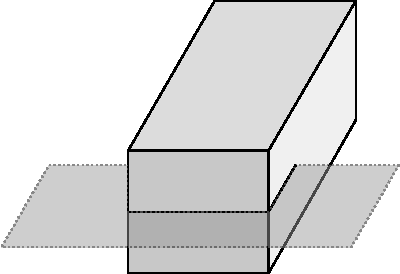
\includegraphics[width=0.7\linewidth]{Figures/Peridigm/Discretization_BondFilters_RectangularPlane}};
% Figure scope
  \begin{scope}[
    x={(image.south east)},
    y={(image.north west)},
  ]
    % Coordinates
    \coordinate (p1)  at (0.005,0.100);
    \coordinate (p2)  at (0.878,0.100);
    \coordinate (p3)  at (0.995,0.397);
    \coordinate (p4)  at (0.125,0.397);
    \coordinate (pn)  at (0.250,0.300);
    
    \coordinate (p1v) at ($(p1)-(0.0,9ex)$);
    \coordinate (p2v) at ($(p2)-(0.0,9ex)$);
    \coordinate (p2s) at ($(p2)+(1em,0.0)$);
    \coordinate (p3s) at ($(p3)+(1em,0.0)$);
    % Dots
    \draw[black,fill=black] (p1) circle (2pt);
    \draw[black]            (p2) circle (2pt);
    \draw[black]            (p3) circle (2pt);
    \draw[black]            (p4) circle (2pt);
    % Nodes
    \node[anchor=east,align=center]  at (p1) {Lower\_\\Left\_\\Corner}; 
    \node[anchor=north,xshift=0.5em] at (p1) {1}; 
    \node[anchor=north]              at (p2) {2};
    \node[anchor=south]              at (p3) {3};
    \node[anchor=south]              at (p4) {4};
    % Arrows
    \draw[-latex,very thick] (p1) -- ($(p1)+(5em,0.0)$) node [below,align=center] {Bottom\_\\Unit\_\\Vector};
    \draw[-latex,very thick] (pn) -- ($(pn)+(0.0,5em)$) node [above] {Normal};
    \draw[latex-latex,very thick] (p1v) -- (p2v) node [midway, anchor=north, align=center] {Bottom\_Length};
    \draw[latex-latex,very thick] (p2s) -- (p3s) node [midway, anchor=west, align=center,xshift=0.5em] {Side\_\\Length};
    % Labels
    \node[anchor=north east]         (modellabel) at (0.4,0.90) {Model};
    \node[anchor=north,align=center] (planelabel) at (0.8,0.03) {Rectangular\\Plane};
    \draw (modellabel) -- (0.55,0.8);
    \draw (planelabel) -- (0.82,0.2);
    % Help grid and labels
    %\pic{myimagegrid};
  \end{scope}
\end{tikzpicture}

  \caption{Bond Filter - Rectangular Plane}
  \label{fig:Peridigm:QRG:Discretization:Tools:BondFilter:RectangularPlane}
\end{figure}

\begin{tabularx}{\linewidth}{lX}
\textit{Lower\_Left\_Corner}  & Point in 3D which defines the origin of the rectangle in its lower left corner, here named ``1''.  \\
\textit{Bottom\_Unit\_Vector} & Vector of unit length in 3D defining the direction along the bottom of the rectangle, here from ``1'' to ``2''.  \\
\textit{Normal}               & Vector in 3D that defines the normal direction of the rectangle. From this and \textit{Bottom\_Unit\_Vector} the vector of the other side of the rectangle, here from ``1'' to ``4'', is calculated internally using the vector or cross product.  \\
\textit{Bottom\_Length}       & Length of the side along \textit{Bottom\_Unit\_Vector}, so the length between ``1'' to ``2'' and ``3'' to ``4''.  \\
\textit{Side\_Length}         & Length of the others two sides, here ``1'' to ``4'' and ``2'' to ``3''.
\end{tabularx}

\levelup{Exemplary input section}

\leveldown{XML-format}

from \verb+/test/regression/PrecrackedPlate/PrecrackedPlate.xml+:

\begingroup
\lstset{breaklines=true}
\begin{code}
<ParameterList name="Discretization">
  <Parameter name="Type" type="string" value="Exodus" />
  <Parameter name="Input Mesh File" type="string" value="Plate.g"/>
  <ParameterList name="Bond Filters">
    <ParameterList name="My First Bond Filter">
      <Parameter name="Type" type="string" value="Rectangular_Plane"/>
      <Parameter name="Normal_X" type="double" value="0.0"/>
      <Parameter name="Normal_Y" type="double" value="1.0"/>
      <Parameter name="Normal_Z" type="double" value="0.0"/>
      <Parameter name="Lower_Left_Corner_X" type="double" value="-10.0"/>
      <Parameter name="Lower_Left_Corner_Y" type="double" value="0.0"/>
      <Parameter name="Lower_Left_Corner_Z" type="double" value="-10.0"/>
      <Parameter name="Bottom_Unit_Vector_X" type="double" value="1.0"/>
      <Parameter name="Bottom_Unit_Vector_Y" type="double" value="0.0"/>
      <Parameter name="Bottom_Unit_Vector_Z" type="double" value="0.0"/>
      <Parameter name="Bottom_Length" type="double" value="10"/>
      <Parameter name="Side_Length" type="double" value="20"/>
    </ParameterList>
  </ParameterList>
</ParameterList>
\end{code}
\endgroup

\levelstay{Free format}

\begingroup
\lstset{breaklines=true}
\begin{code}
Discretization
  ...
  Bond Filters
    bond_filter-1
      Type "Rectangular_Plane"
      Normal_X 0.0
      Normal_Y -1.0
      Normal_Z 0.0
      Lower_Left_Corner_X -0.1
      Lower_Left_Corner_Y 0.0
      Lower_Left_Corner_Z -0.1
      Bottom_Unit_Vector_X 0.0
      Bottom_Unit_Vector_Y 0.0
      Bottom_Unit_Vector_Z 1.0
      Bottom_Length 0.2
      Side_Length 10.1
\end{code}
\endgroup

\levelstay{YAML format}

-

\levelup{List of examples}

\begin{itemize}[noitemsep]
%   \item From \texttt{examples/}:
%   \begin{itemize}[noitemsep]
%     \item \texttt{examples/tensile_test/tensile_test.peridigm}
%   \end{itemize}
  \item From \texttt{test/regression/}:
  \begin{itemize}[noitemsep]
    \item \texttt{PrecrackedPlate/PrecrackedPlate.xml}
    \item \texttt{PrecrackedPlateTwoCracks/PrecrackedPlateTwoCracks.xml}
  \end{itemize}
%   \item From \texttt{test/verification/}:
%   \begin{itemize}[noitemsep]
%     \item \texttt{Contact_Friction/Contact_Friction.xml}
%   \end{itemize}
\end{itemize}
% \begin{itemize}[noitemsep]
%   \item \texttt{/test/regression/PrecrackedPlate/PrecrackedPlate.xml}
%   \item \texttt{/test/regression/PrecrackedPlateTwoCracks/PrecrackedPlateTwoCracks.xml}
% \end{itemize}
